\section{Desenvolvimento}

\subsection{Formulação da base de dados}

\par Na abordagem executada para o problema, foi feita uma combinação de bases de dados de origem governamental para fornecer substrato para resolução do problema.

\subsubsection{Bases utilizadas}

\par Primeiramente, a fim de se obter uma base detentora de conhecimento acerca dos dados do sistema educacional brasileiro, foi feita a integração de bases do censo escolar de 2021 sobre indicadores educacionais de dois níveis de ensino no país, ensino médio e ensino fundamental, como as taxas de rendimento escolares e o grau de esforço docente, realizado pelo \textbf{INEP}, e da base de dados municipais fornecida pelo \textbf{IBGE} do mesmo ano, integrando informações como o PIB e o PIB per capta municipais à base principal. Cada exemplo na base representa uma escola no território nacional, com atributos sobre município, dependência e categoria da entidade.

\subsubsection{Imputação de dados}

\par Com o intuito de tratar os dados faltantes das bases integradas foi feita a imputação de dados por meio do algoritmo do \textit{KNN}, com parâmetro K igual a cinco, considerando os objetos que pertenciam à mesma unidade federativa nacional a fim de se obter um resultado condizente para os atributos ausentes nas bases primitivas sem exigir recursos computacionais e tempo excessivamente elevados. Assim, foi feita a média entre os atributos dos cinco objetos mais similares ao exemplar com ausência de certos atributos tratar a problemática.

\subsubsection{Desenvolvimento de atributo alvo}

\par Para que a base de dados tenha um atributo alvo que englobe as taxas de evasão em ambos os níveis de ensino analisados, médio e fundamental, foi feita a taxa total de evasão da escola com base na quantidade de turmas existentes na unidade de ensino, na média de alunos por turma e pela taxa de evasão escolar em cada nível de ensino. Portanto, o atributo alvo foi calculado pela equação:

\begin{equation*}
    \frac{Alunos/Turma_{EF} \cdot Turmas_{EF} \cdot Evas\tilde{a}o_{EF} + Alunos/Turma_{EM} \cdot Turmas_{EM} \cdot Evas\tilde{a}o_{EM}}{Alunos/Turma_{EF} \cdot Turmas_{EF} + Alunos/Turma_{EM} \cdot Turmas_{EM}}
\end{equation*}

\par Dessa maneira, as taxas de evasão total de cada instituição de ensino são categorizadas da seguinte forma:

\[
\begin{cases} 
\text{Baixa} & \text{se } Evas\tilde{a}o < 5 \\
\text{Moderada} & \text{se } 5 \leq Evas\tilde{a}o \leq 10 \\
\text{Alta} & \text{se } Evas\tilde{a}o > 10 
\end{cases}
\]

\subsection{Análise exploratória de dados}

\par Com o intuito de se obter uma maior noção sobre o conjunto de dados do problema, faz-se uma análise exploratória da base.

\subsubsection{Distribuição da base}

\par A fim de analisar a distribuição entre as classes de evasão escolar, lança-se mão do histograma de categorias do conjunto de dados analisados.

\begin{figure}[H]
    \centering
    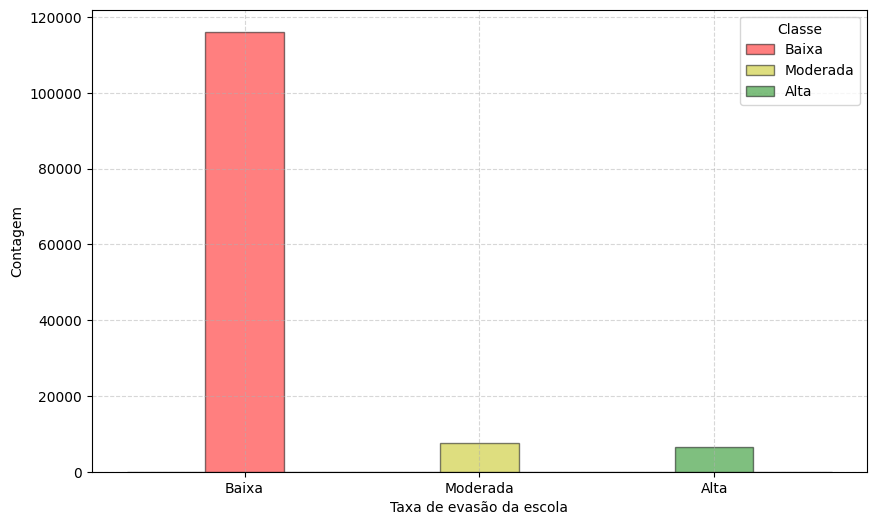
\includegraphics[scale = 0.6]{Graphics/Hist-Eva.png}
    \caption{Histograma das categorias de evasão da base.}
    \label{fig:hist-eva}
\end{figure}

\par Vista a distribuição explicitada na \textbf{Figura 1}, vê-se que há um desbalanceamento significativo entre as categorias de evasão escolar, sendo a classe majoritária a classe Baixa. Assim, é razoável inferir que haverá um enviesamento no treinamento do modelo, beneficiando a classificação como a categoria com mais representantes, fator que faz necessário métodos de amostragem e de treinamento que contornem o problema.

\par A distribuição também mascara outra problemática do sistema educacional brasileiro, porém, sendo logístico, de que cerca de 79,5\% das escolas que possuem taxa de evasão baixa, não apresentam turmas no ensino médio. Portanto, dado que a taxa de evasão no ensino fundamental é naturalmente mais baixa, a taxa de evasão da maioria das entidades se configura como baixa devido à falta de estrutura, outro problema do sistema educacional nacional.

\begin{figure}
    \centering
    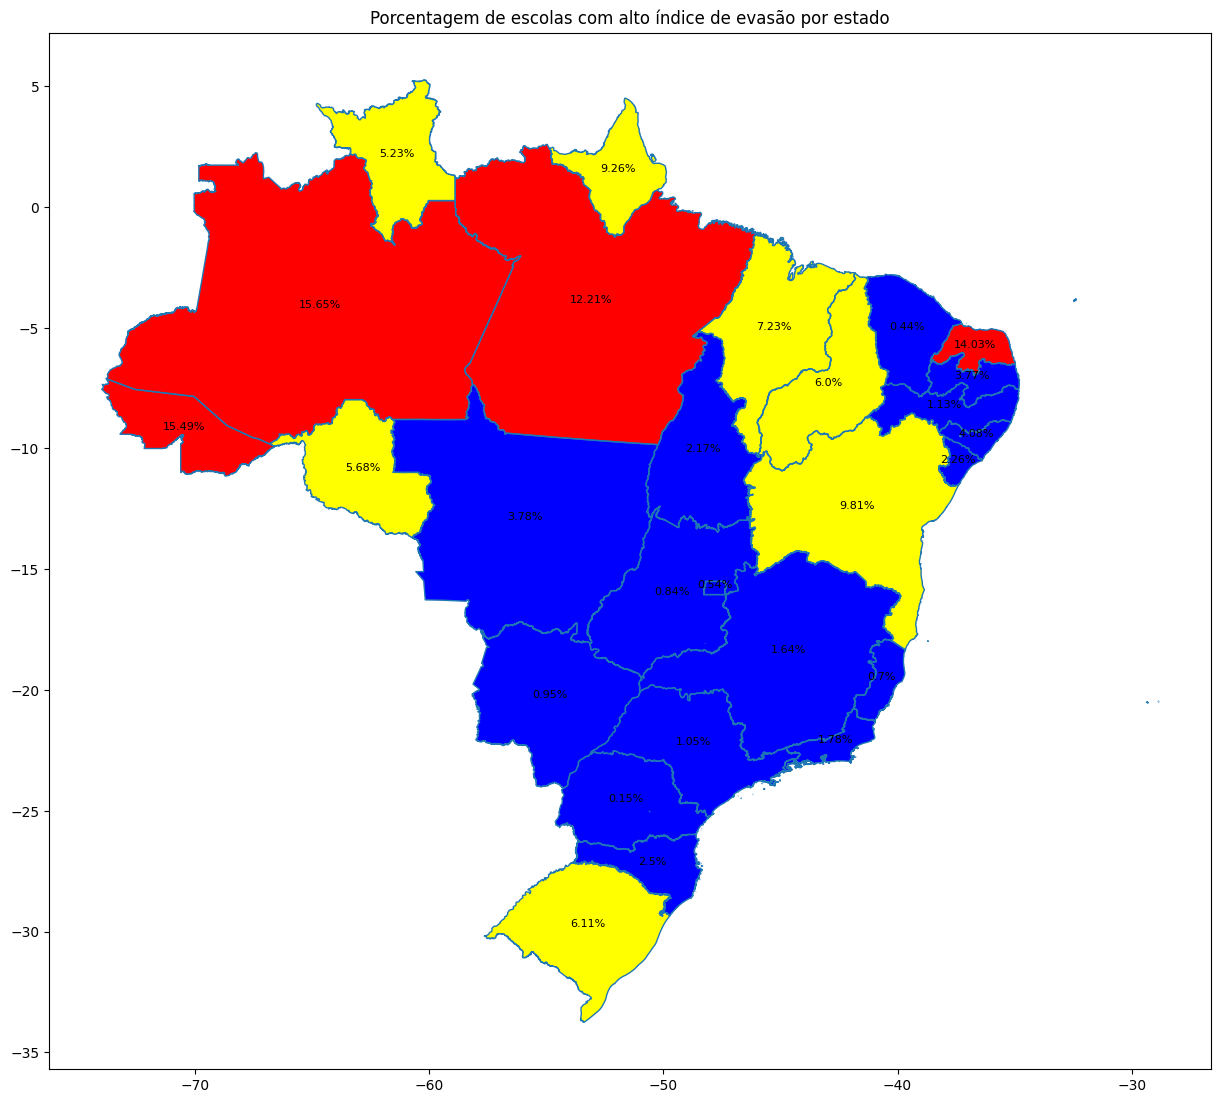
\includegraphics[scale = 0.3]{Graphics/Mapa.png}
    \caption{Mapa com taxa de escolas com índice de evasão alto.}
    \label{fig:enter-label}
\end{figure}

\subsubsection{Mapa de calor}

\par Com o intuito de se observar a correlação das variáveis utilizadas no problema de aprendizado, faz-se uso do mapa de calor para as correlações com os coeficientes de Pearson e de Kendall.

\begin{figure}[H]
    \centering
    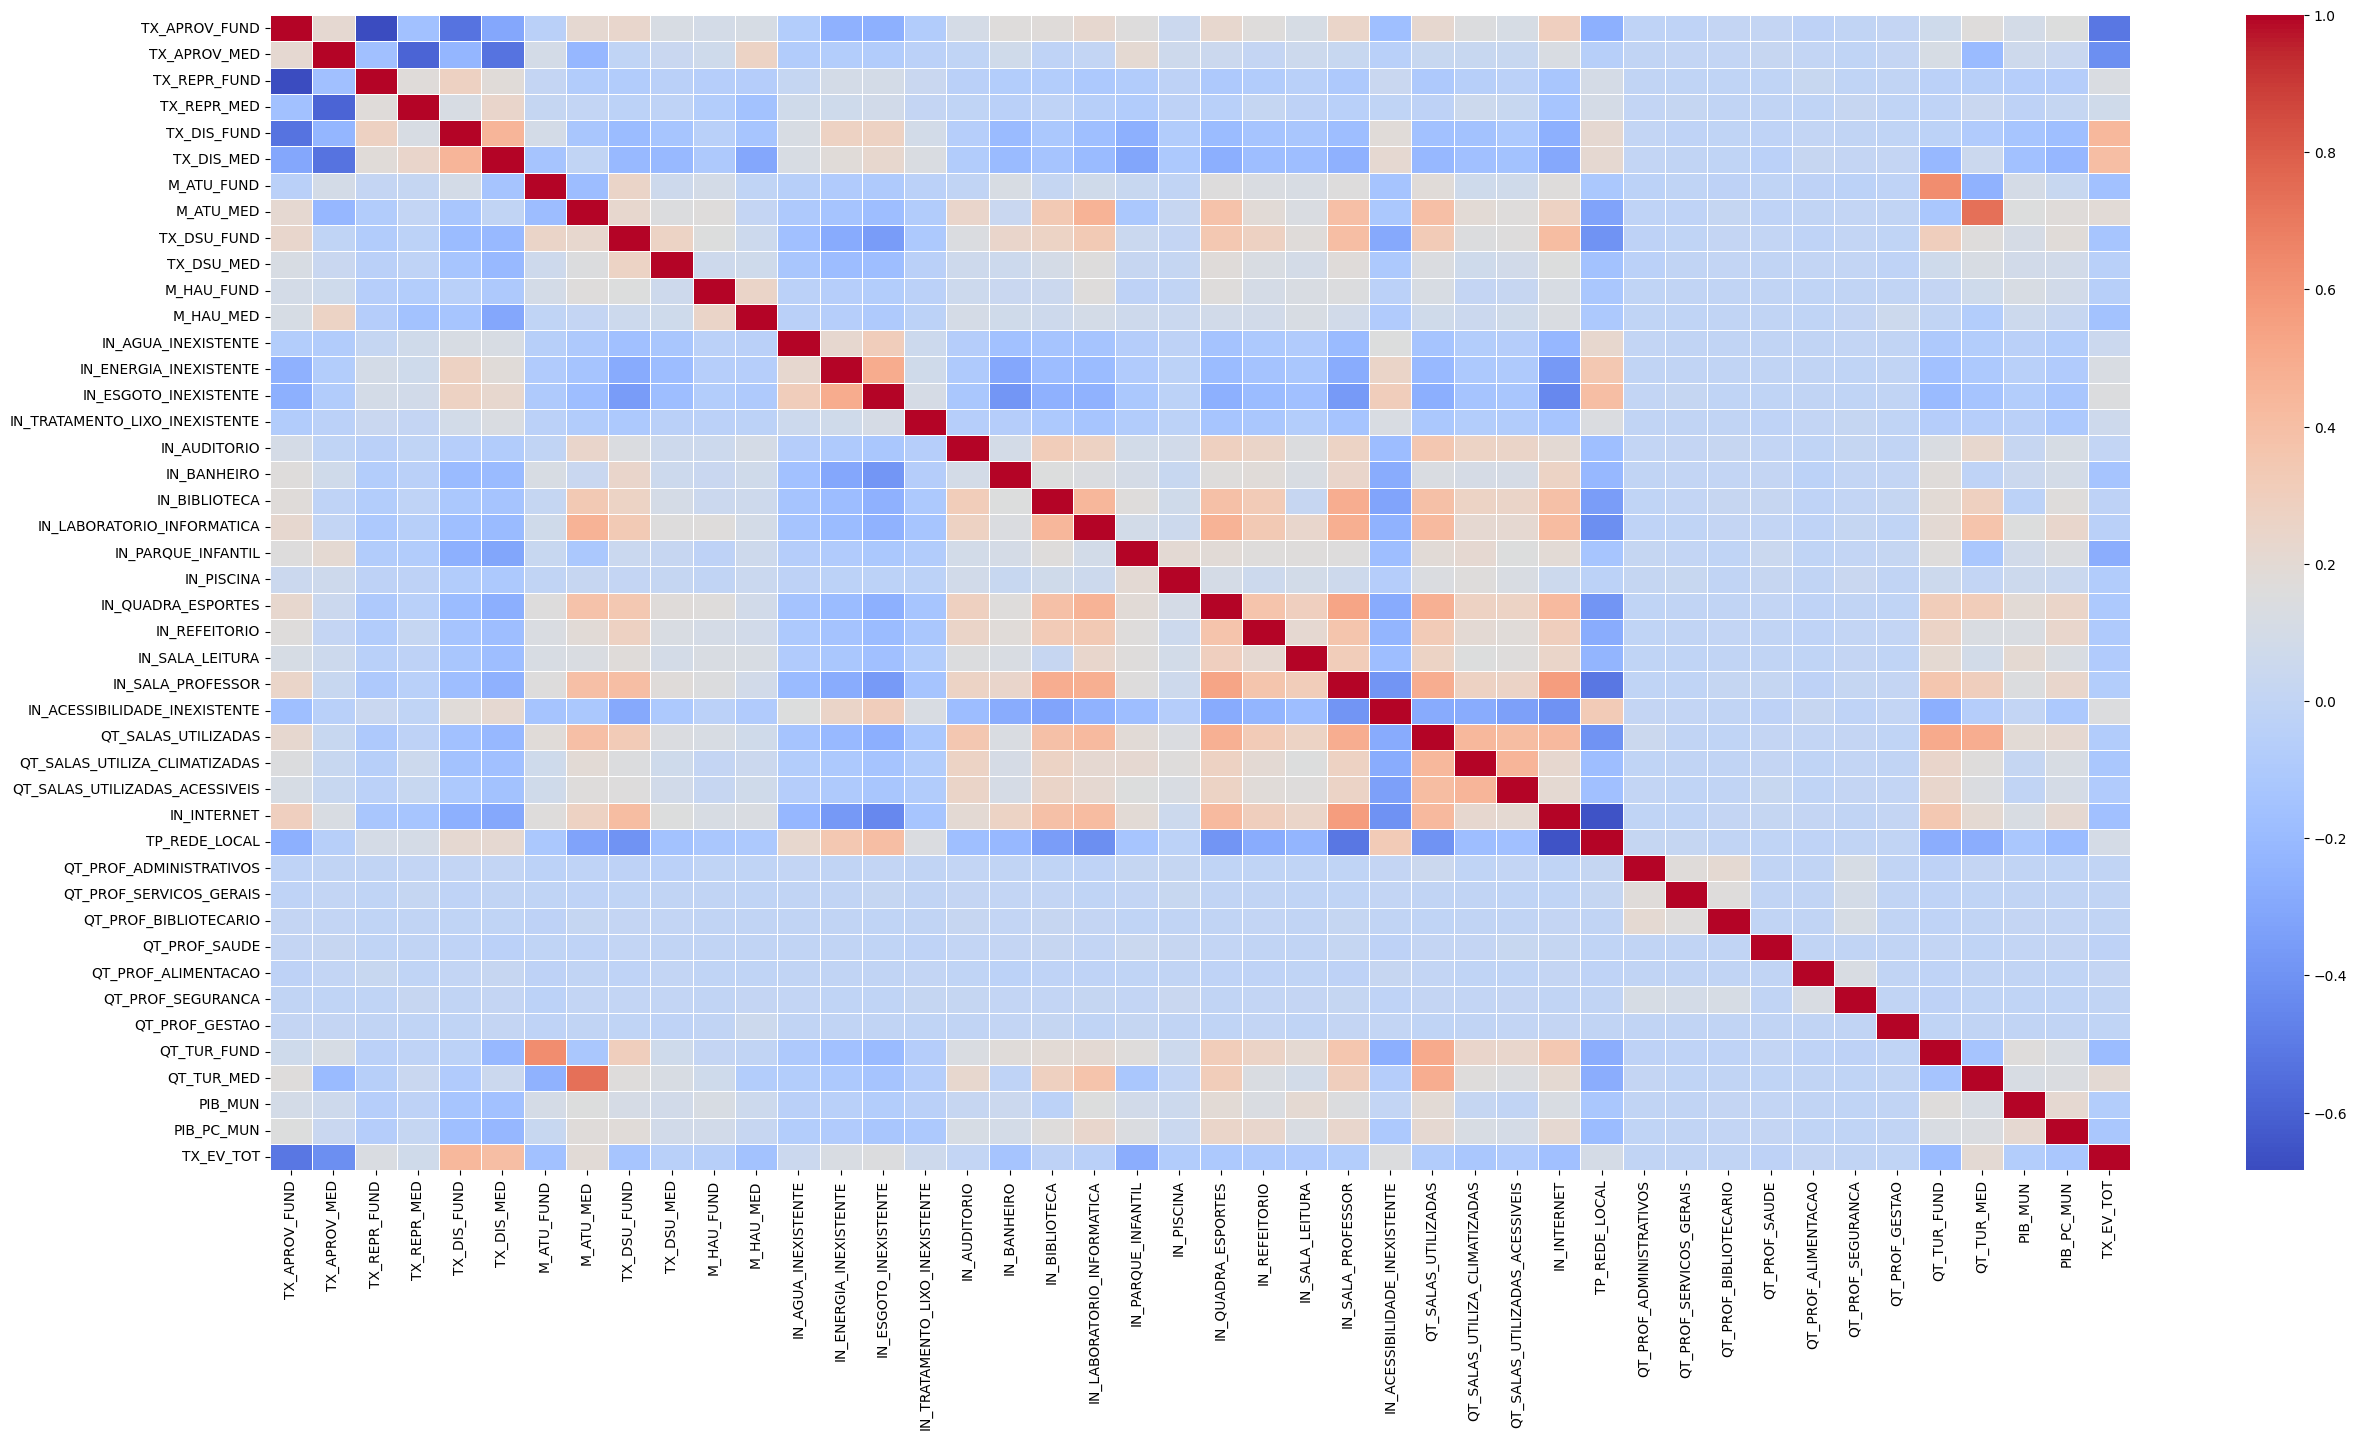
\includegraphics[scale = 0.25]{Graphics/Heatmap-Pearson.png}
    \caption{Mapa de correlação entre os atributos da base com coeficiente de Pearson.}
    \label{fig:heatmap}
\end{figure}

\begin{figure}[H]
    \centering
    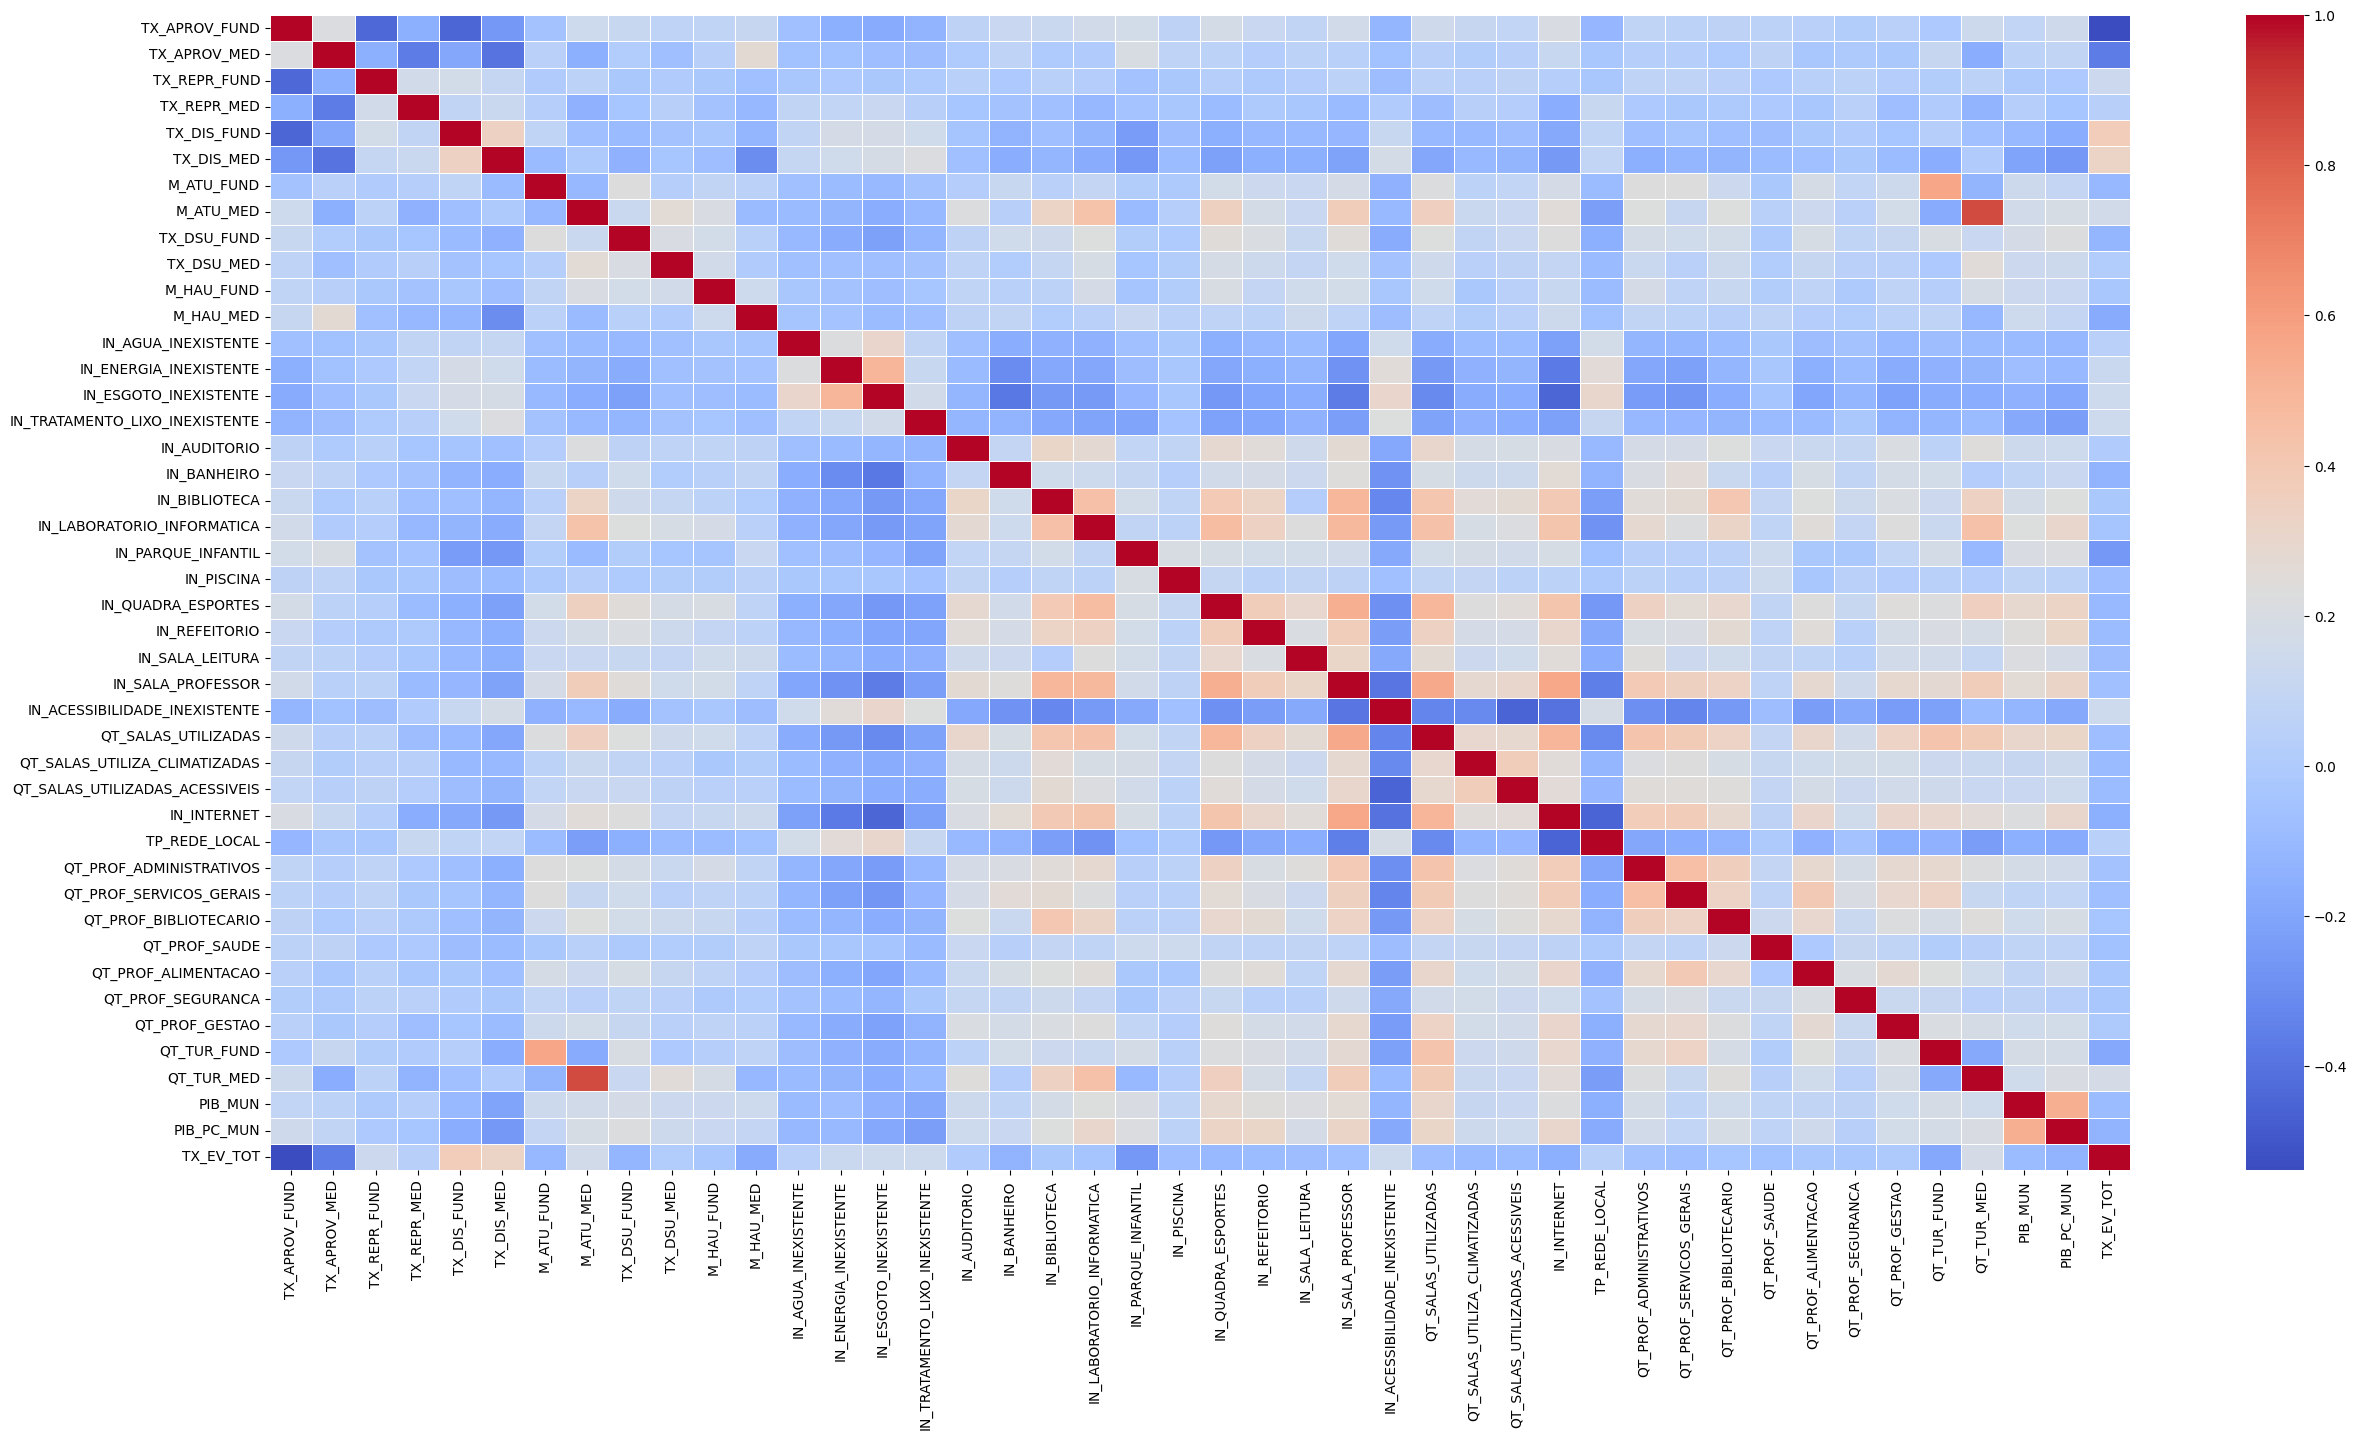
\includegraphics[scale = 0.25]{Graphics/Heatmap-Kendall.png}
    \caption{Mapa de correlação entre os atributos da base com coeficiente de Kendall.}
    \label{fig:heatmap}
\end{figure}

\par A partir dos gráficos de correlação nos mapas de calor, é possível inferir que há poucos casos de variáveis que apresentam correlação significativamente forte, seja de maneira diretamente ou inversamente proporcional. Desse modo, é razoável concluir que os dados são pouco relacionados, fator que corrobora a hipótese de que não há uma redundância considerável entre os atributos e que não há urgência na redução da dimensionalidade da base, com cada característica representando um aspecto distinto de cada instituição de ensino.

\subsubsection{Gráficos de dispersão}

Com o intuito de se obter uma visualização mais precisa da correlação entre os atributos, faz-se uso dos gráficos de dispersão da base.

\begin{figure}[H]
    \centering
    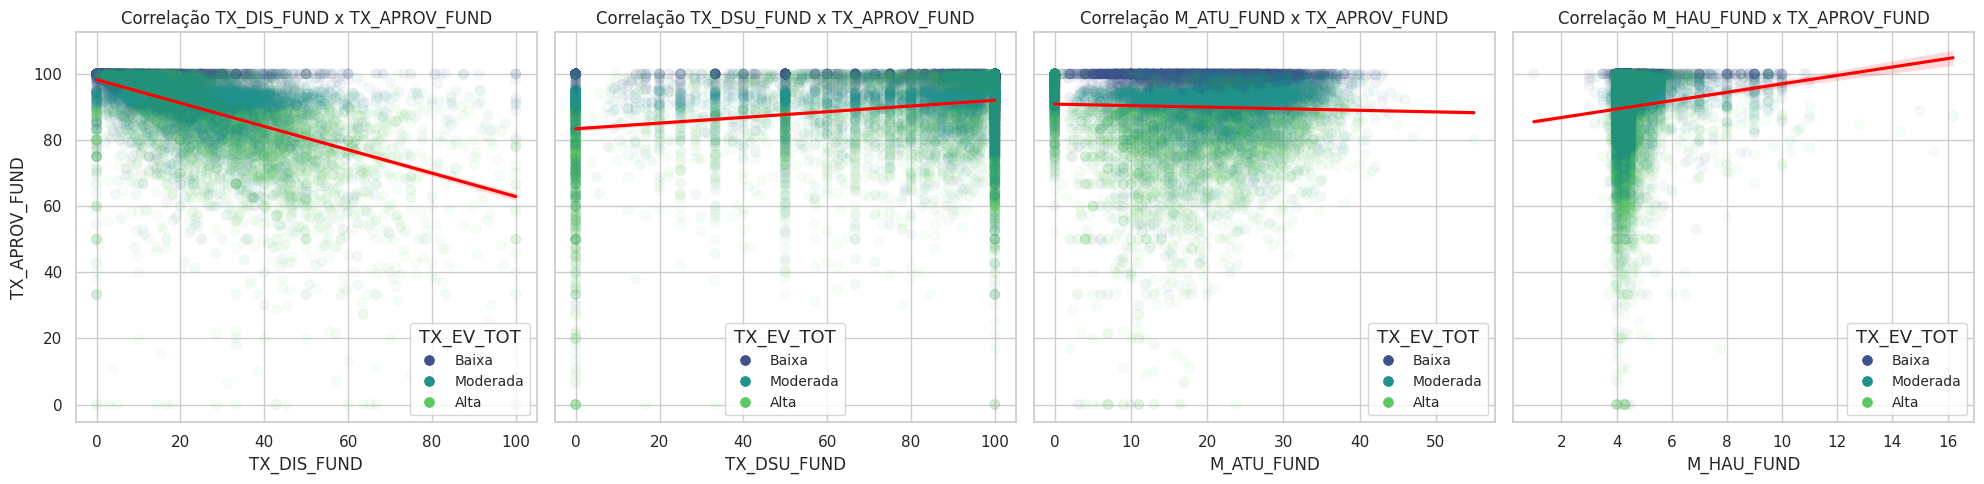
\includegraphics[scale = 0.3]{Graphics/Disp-Fund.png}
    \caption{Gráficos de dispersão entre as taxas do ensino fundamental.}
    \label{fig:disp-fund}
\end{figure}

\par Entre as taxas de rendimento do ensino fundamental, é razoável inferir que apenas a taxa de distorção idade-série apresenta uma correlação significativa com a taxa de aprovação no nível de ensino, fator que implica uma forte relação entre as características.

\begin{figure}[H]
    \centering
    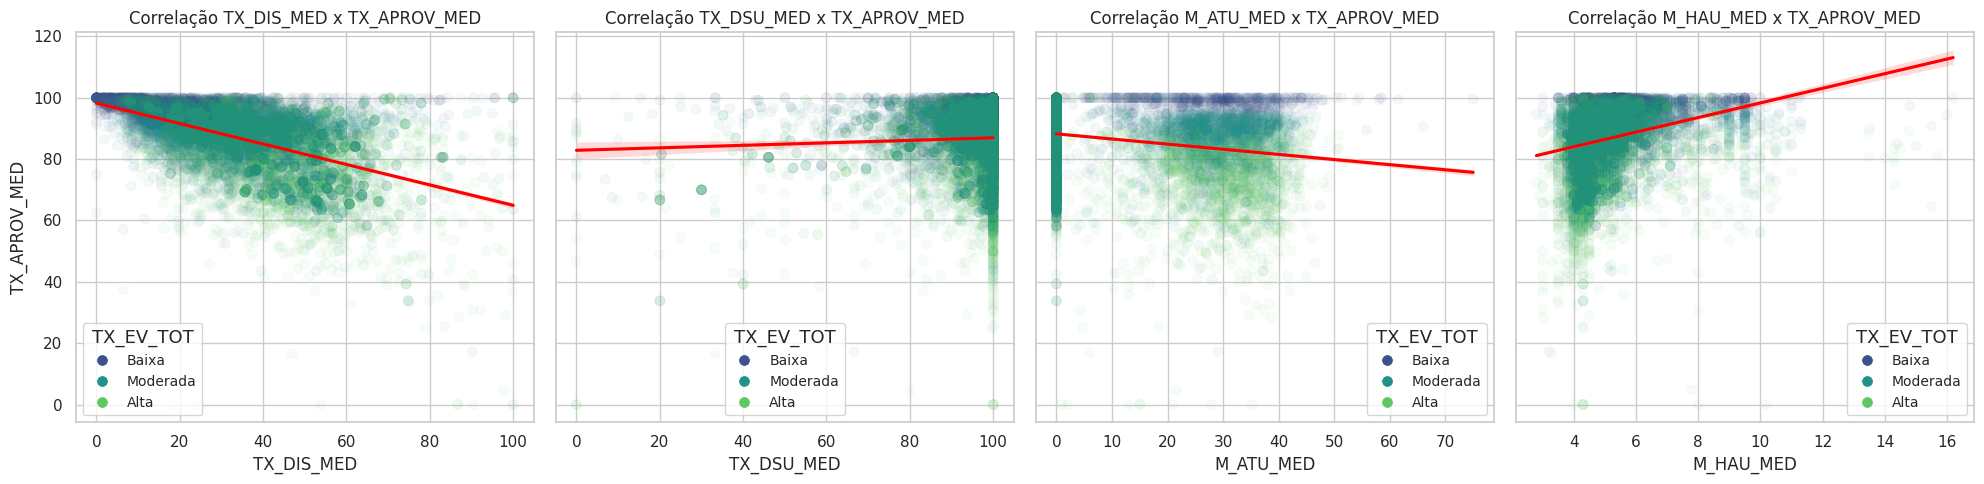
\includegraphics[scale = 0.3]{Graphics/Disp-Med.png}
    \caption{Gráficos de dispersão entre as taxas do ensino fundamental.}
    \label{fig:disp-med}
\end{figure}

\par Entre as taxas de rendimento do ensino médio, é possível tomar uma conclusão análoga ao ensino fundamental em que a taxa de aprovação tem uma relação mais forte com a taxa de distorção idade-série em detrimento das outras características observadas.

\par Os gráficos de dispersão, em consonância com o mapa de calor, corrobora a ideia de que as variáveis não apresentam redundância significativa e que a dimensionalidade da base não evidencia problema gritante.

\subsubsection{Gráficos de violino}

\par A fim de observar a concentração de valores de alguns atributos entre as categorias da base, são utilizados gráficos violino para que seja possível visualizar as tendências de acúmulo entre os dados.

\begin{figure}[H]
    \centering
    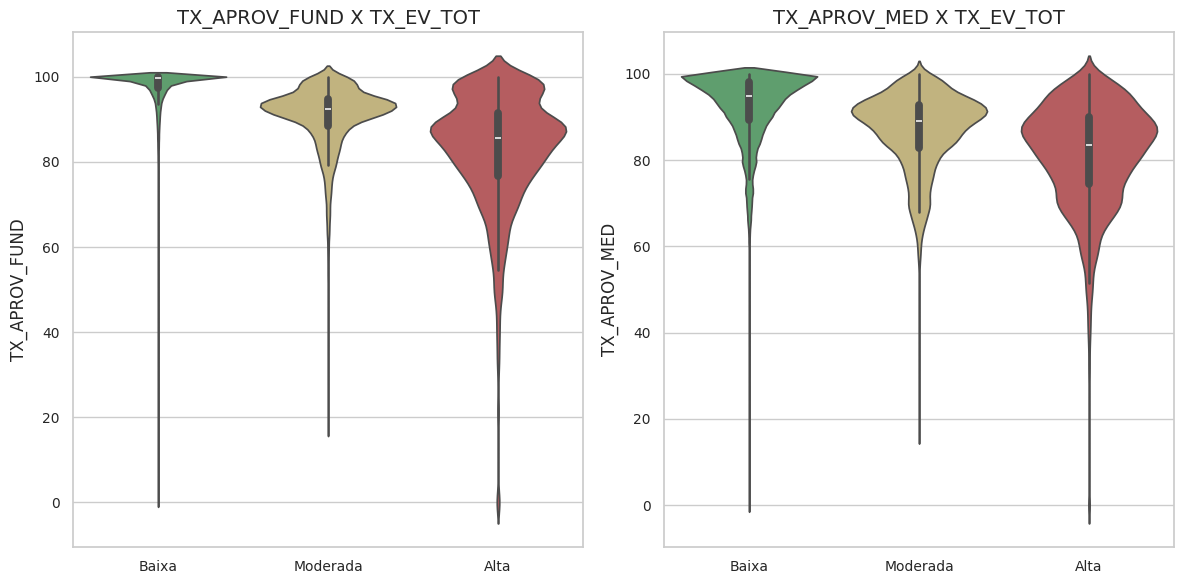
\includegraphics[scale = 0.4]{Graphics/Vio-Aprov.png}
    \caption{Gráficos de violino da taxa de aprovação para cada categoria.}
    \label{fig:enter-label}
\end{figure}

\par A partir da \textbf{Figura 4}, vê-se que a distribuição da taxa de aprovação dentre as classes segue a intuição de que à medida de que a evasão escolar aumenta a taxa de reprovação é reduzido. Ademais, analisando os gráficos individualmente, vê-se que a redução taxa de aprovação no ensino fundamental se mostrou ligeiramente mais significativa para a distinção entre as taxas mais altas.

\begin{figure}[H]
    \centering
    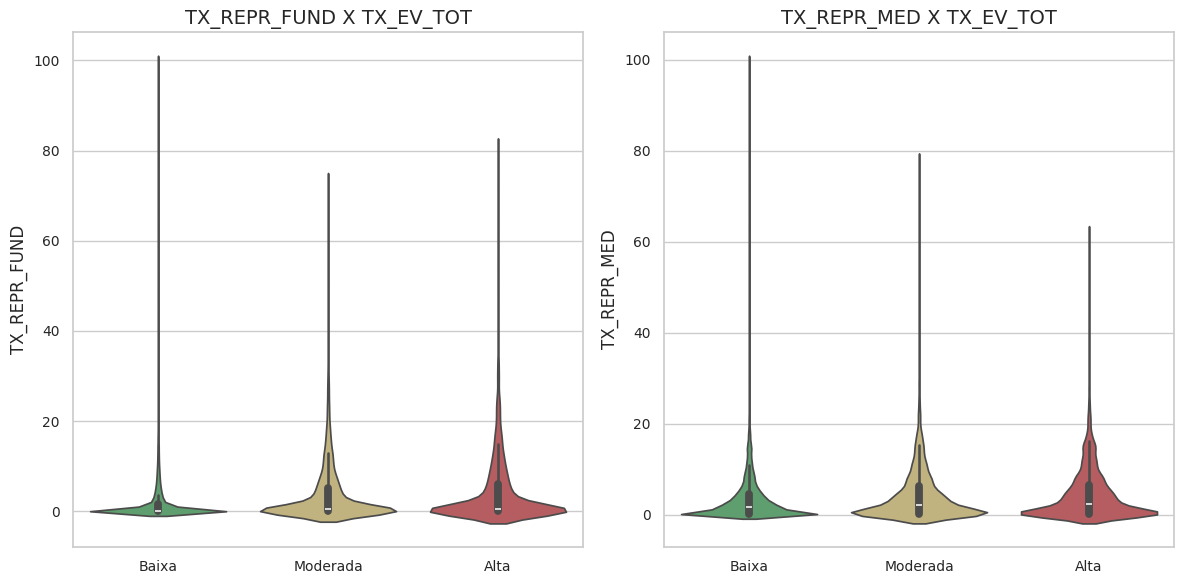
\includegraphics[scale = 0.4]{Graphics/Vio-Repr.png}
    \caption{Gráficos de violino da taxa de reprovação para cada categoria.}
    \label{fig:enter-label}
\end{figure}

\par Tomando como substrato de análise a \textbf{Figura 5}, não é tão razoável inferir uma proporcionalidade visual tão clara da reprovação nos níveis de ensino à medida que a taxa de evasão aumenta, porém, ainda é possível observar um ligeiro incremento da reprovação em categorias mais altas.

\begin{figure}[H]
    \centering
    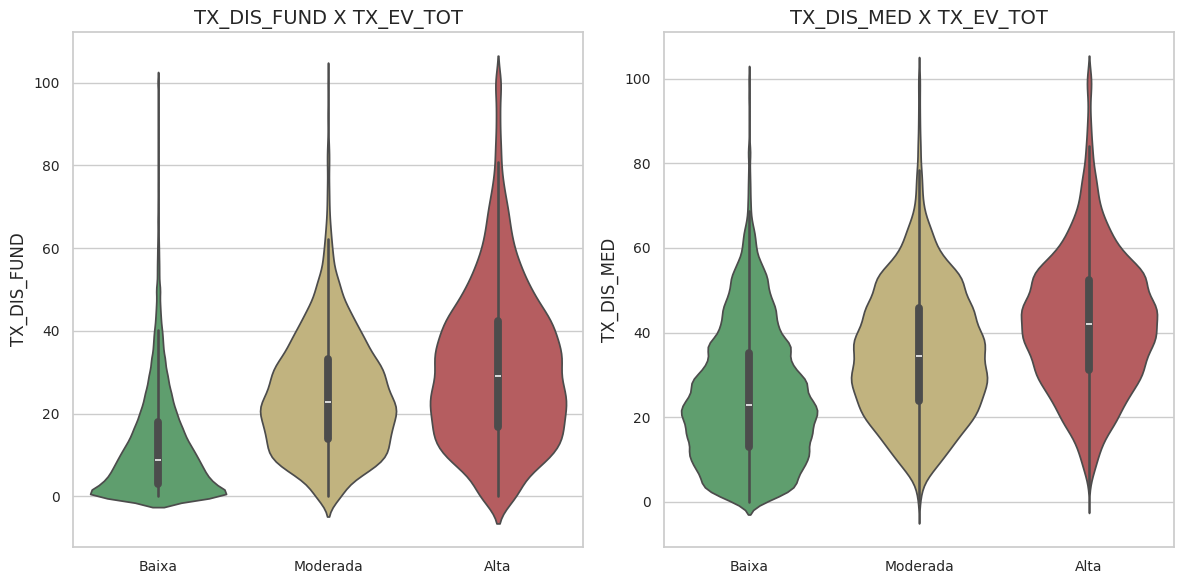
\includegraphics[scale = 0.4]{Graphics/Vio-DIS.png}
    \caption{Gráficos de violino da taxa de distorção idade-série para cada categoria.}
    \label{fig:enter-label}
\end{figure}

\par Por intermédio da \textbf{Figura 3}, percebe-se uma notável relação do indicador de distorção idade-série com a taxa de evasão, apresentando um aumento considerável proporcional ao atributo alvo. Além disso, analogamente aos índices de aprovação, infere-se que a evasão se mostrou mais sensível ao incremento da taxa de distorção idade-série do ensino fundamental em detrimento do ensino médio, fator que evidencia uma significativa relevância do nível de ensino no sistema educacional como um todo.

\subsection{Modelagem}

\subsubsection{Amostragem}

\par A fim de reduzir os custos computacionais e diminuir o tempo de execução durante a etapa de treinamento, a abordagem acatada foi utilizar uma amostra da base com cerca de 10\% dos objetos totais do conjunto original.

\par Graças ao alto grau de desbalanceamento da base completa, a etapa de amostragem foi abordada de duas formas diferentes que serão exploradas: uma amostra será artificialmente balanceada, ou seja, os exemplos serão escolhidos dada uma proporção estabelecida de exemplares de cada classe, a proporção escolhida foi uniforme entre as categorias, um terço de cada classe, sendo que os exemplos dentro de cada segmento serão escolhidos aleatoriamente, e a outra amostra será desenvolvida com exemplos aleatórios, sendo assim, a proporção original será, teoricamente, mantida.

\subsubsection{Random Forest}

\par Random Forest é um algoritmo de aprendizado de máquina baseado em árvores de decisão que utiliza o conceito de ensemble learning para melhorar a precisão e robustez das previsões. Tal técnica agrega múltiplas árvores de decisão, técnica de \textit{bagging}, para aprimorar a acurácia do modelo final e reduzir o risco de \textit{overfitting}.

\par Suas vantagens incluem a redução do risco de overfitting, pois combina múltiplas árvores de decisão, o cálculo da importância dos atributos, fornecendo uma medida de quanto cada um contribui para a predição e sua versatilidade, já que pode ser usado tanto para classificação quanto para regressão.

\par No contexto do problema apresentado, o Random Forest pode ser utilizado tanto na classificação das taxas de evasão escolar quanto na identificação dos atributos mais importantes que influenciam essa taxa ajudando na tomada de decisões para mitigar o problema.

\par Para o treinamento do modelo com Random Forest, foi utilizado o método de divisão do K-Fold com K igual a dez.

\subparagraph{Amostra balanceada} 

\

\par Primeiramente, treina-se o modelo com a Random Forest na amostra de dados balanceada.

\begin{figure}[H]
    \centering
    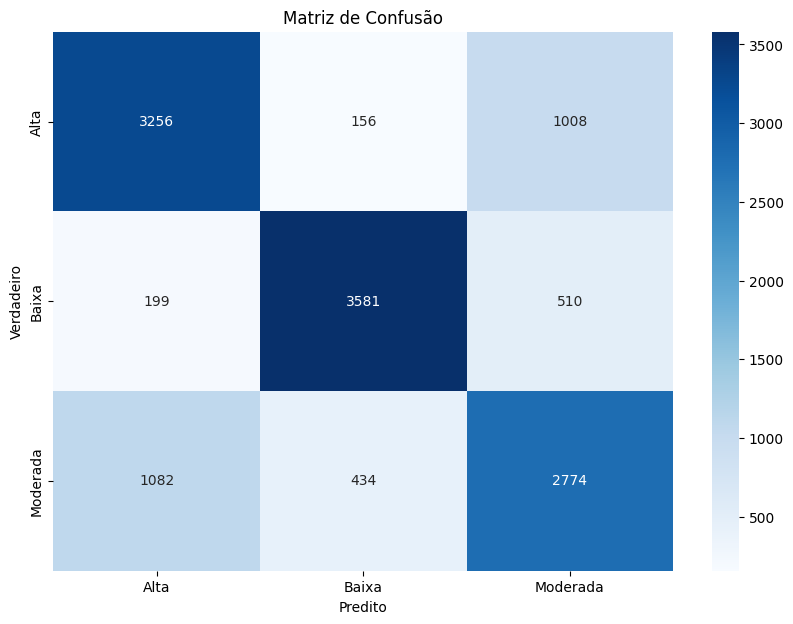
\includegraphics[scale = 0.4]{Graphics/Mat-Conf-Rand-Bal.png}
    \caption{Matriz de confusão para o algoritmo da Random Forest na amostra balanceada.}
    \label{fig:enter-label}
\end{figure}

\begin{table}[H]
    \centering
    \begin{tabular}{lcc}
        \toprule
        \textbf{Classe} & \textbf{Precisão} & \textbf{Recall} \\
        \midrule
        Alta      & 0.72 & 0.74 \\
        Baixa     & 0.86 & 0.83 \\
        Moderada  & 0.65 & 0.65 \\
        \midrule
        \textbf{Acurácia} & \multicolumn{2}{c}{0.74} \\
        \bottomrule
    \end{tabular}
    \caption{Tabela de precisão e recall para as classes alta, moderada e baixa para a Random Forest na amostra balanceada.}
\end{table}

\paragraph{Amostra aleatória}.

\begin{figure}[H]
    \centering
    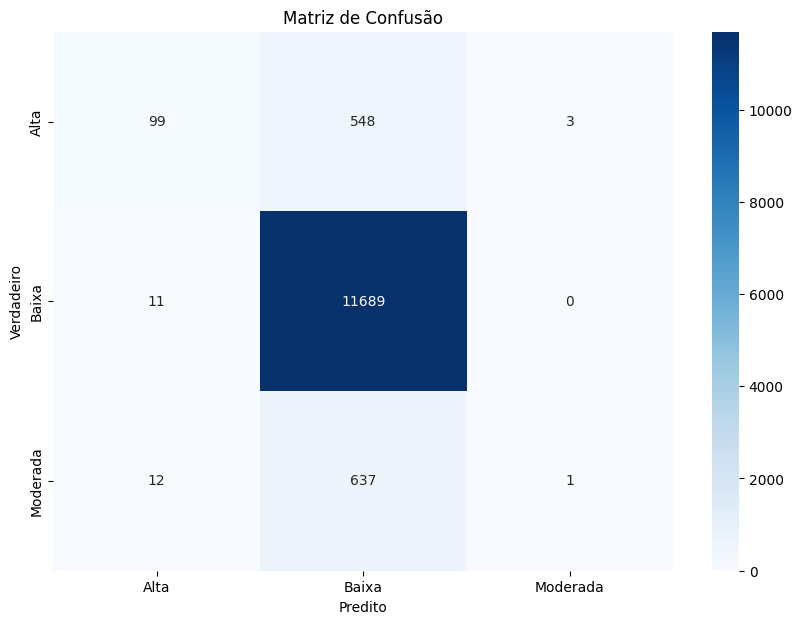
\includegraphics[scale = 0.4]{Graphics/Mat-Conf-Rand-Ale.png}
    \caption{Matriz de confusão para o algoritmo da Random Forest na amostra balanceada.}
    \label{fig:enter-label}
\end{figure}

\begin{table}[H]
    \centering
    \begin{tabular}{lcc}
        \toprule
        \textbf{Classe} & \textbf{Precisão} & \textbf{Recall} \\
        \midrule
        Alta      & 0.81 & 0.15 \\
        Baixa     & 0.91 & 1.00 \\
        Moderada  & 0.25 & 0.00 \\
        \midrule
        \textbf{Acurácia} & \multicolumn{2}{c}{0.91} \\
        \bottomrule
    \end{tabular}
    \caption{Tabela de precisão e recall para as classes alta, moderada e baixa para a Random Forest na amostra aleatória.}
\end{table}

\subsubsection{Redes Neurais}

\par Redes Neurais são modelos inspirados no funcionamento do cérebro humano, capazes de identificar padrões complexos e não-lineares nos dados, tornando-os ideais para prever a evasão escolar com alta precisão. As estruturas são capazes de modelar relações complexas e não lineares nos dados, podem ser escaladas com camadas adicionais e neurônios para aumentar a capacidade de aprendizado e, quando bem treinadas, podem generalizar bem em dados não vistos, assumindo que não há overfitting.

\par Para o nosso problema, as redes neurais podem ser usadas para classificar as taxas de evasão escolar com alta precisão, especialmente quando os dados são complexos e não lineares, além da detecção de padrões complexos nos dados que podem não ser evidentes com métodos mais simples.

\paragraph{Amostra balanceada}.

\begin{figure}[H]
    \centering
    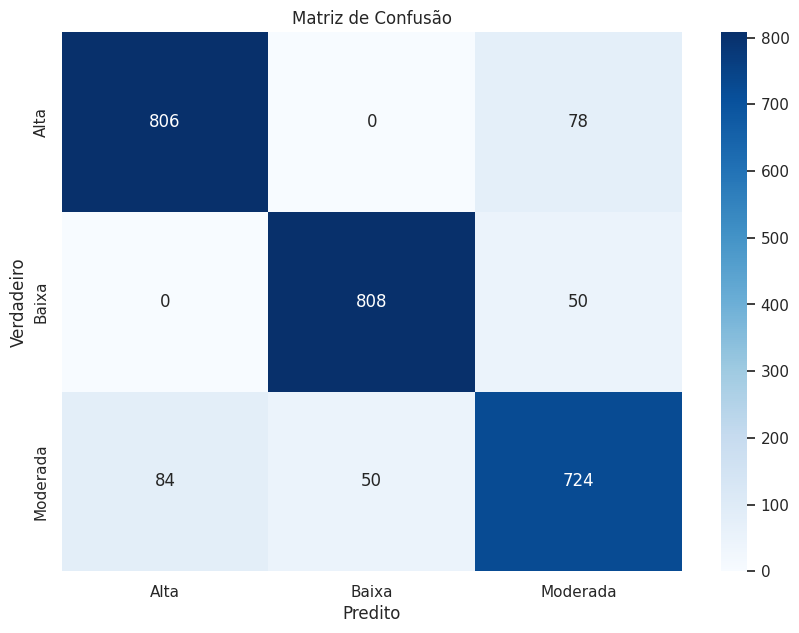
\includegraphics[scale = 0.4]{Graphics/Mat-Conf-Rede-Bal.png}
    \caption{Matriz de confusão para o algoritmo da rede neural na amostra balanceada.}
    \label{fig:enter-label}
\end{figure}

\begin{table}[H]
    \centering
    \begin{tabular}{lcc}
        \toprule
        \textbf{Classe} & \textbf{Precisão} & \textbf{Recall} \\
        \midrule
        Alta      & 0.91 & 0.91 \\
        Baixa     & 0.94 & 0.94 \\
        Moderada  & 0.85 & 0.85 \\
        \midrule
        \textbf{Acurácia} & \multicolumn{2}{c}{0.90} \\
        \bottomrule
    \end{tabular}
    \caption{Tabela de precisão e recall para as classes alta, moderada e baixa para a rede neural na amostra balanceada.}
\end{table}

\paragraph{Amostra aleatória}.

\begin{figure}[H]
    \centering
    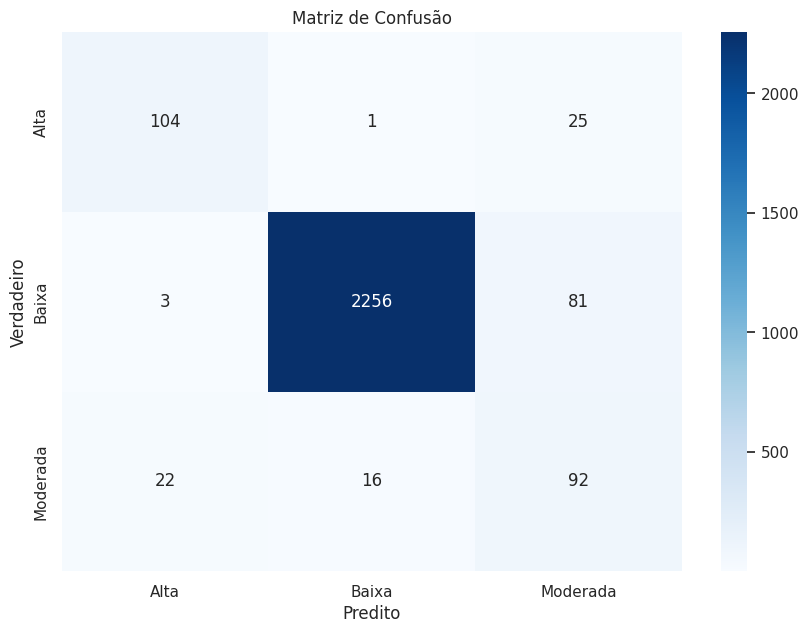
\includegraphics[scale = 0.4]{Graphics/Mat-Conf-Rede-Ale.png}
    \caption{Matriz de confusão para o algoritmo da rede neural na amostra balanceada.}
    \label{fig:enter-label}
\end{figure}

\begin{table}[H]
    \centering
    \begin{tabular}{lcc}
        \toprule
        \textbf{Classe} & \textbf{Precisão} & \textbf{Recall} \\
        \midrule
        Alta      & 0.81 & 0.80 \\
        Baixa     & 0.99 & 0.96 \\
        Moderada  & 0.46 & 0.71 \\
        \midrule
        \textbf{Acurácia} & \multicolumn{2}{c}{0.94} \\
        \bottomrule
    \end{tabular}
    \caption{Tabela de precisão e recall para as classes alta, moderada e baixa para a rede neural na amostra aleatória.}
\end{table}

\section{Análise dos Resultados}

\subsection{Análise geral}

\par A partir dos resultados da modelagem, é possível inferir que o treinamento sobre uma amostra aleatória, apesar de elevar a acurácia geral do modelo, reduz significantemente a sensibilidade da estrutura preditiva em relação a instituições de ensino que apresentam uma taxa de evasão mais elevado, fator observado pelos baixos valores de recall das categorias de evasão mais altas nos resultados, as quais são as entidades alvo do estudo, portanto, as amostras apresentam menor eficiência para o propósito da tarefa de predição que é identificar os principais atributos que implicam fragilização de uma escola ou de um município no geral.

\par Além disso, é possível extrair as importâncias dadas para cada atributo por meio do algoritmo da Random Forest.

\begin{figure}[H]
    \centering
    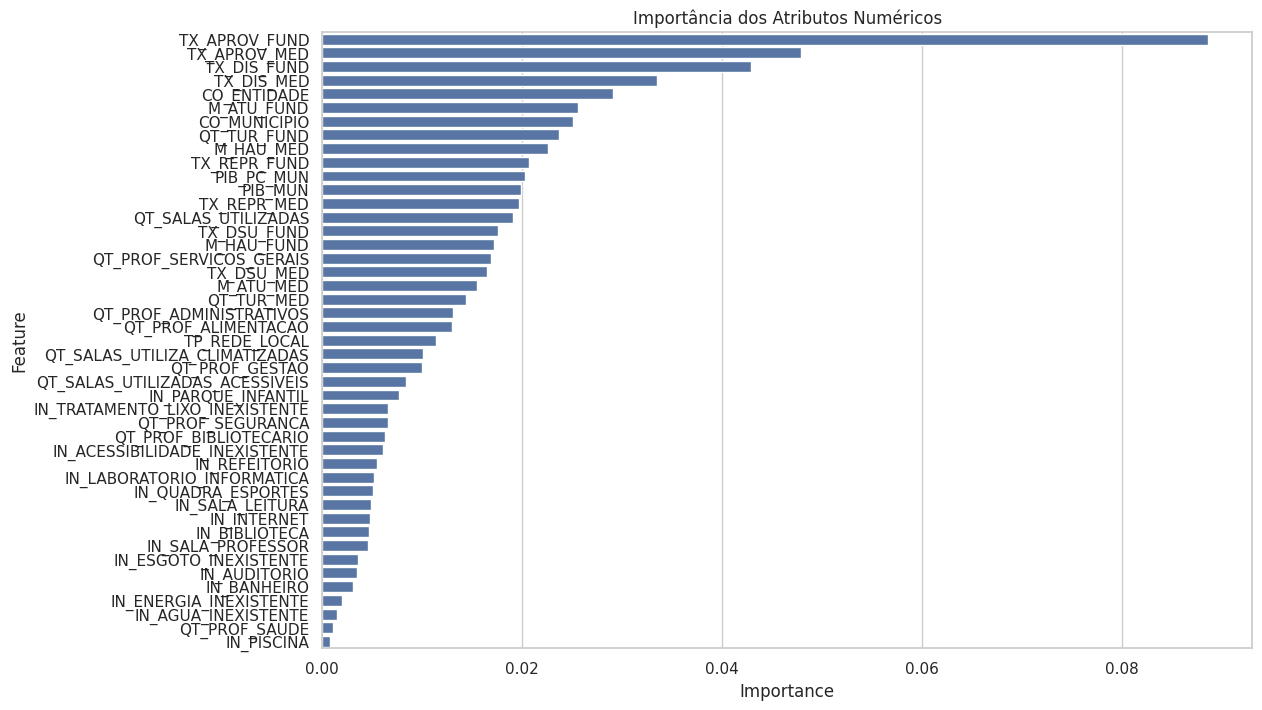
\includegraphics[scale = 0.4]{Graphics/Import-Bal.png}
    \caption{Importância dos atributos atribuídas pela Random Forest na amostragem balanceada.}
    \label{fig:enter-label}
\end{figure}

\begin{figure}[H]
    \centering
    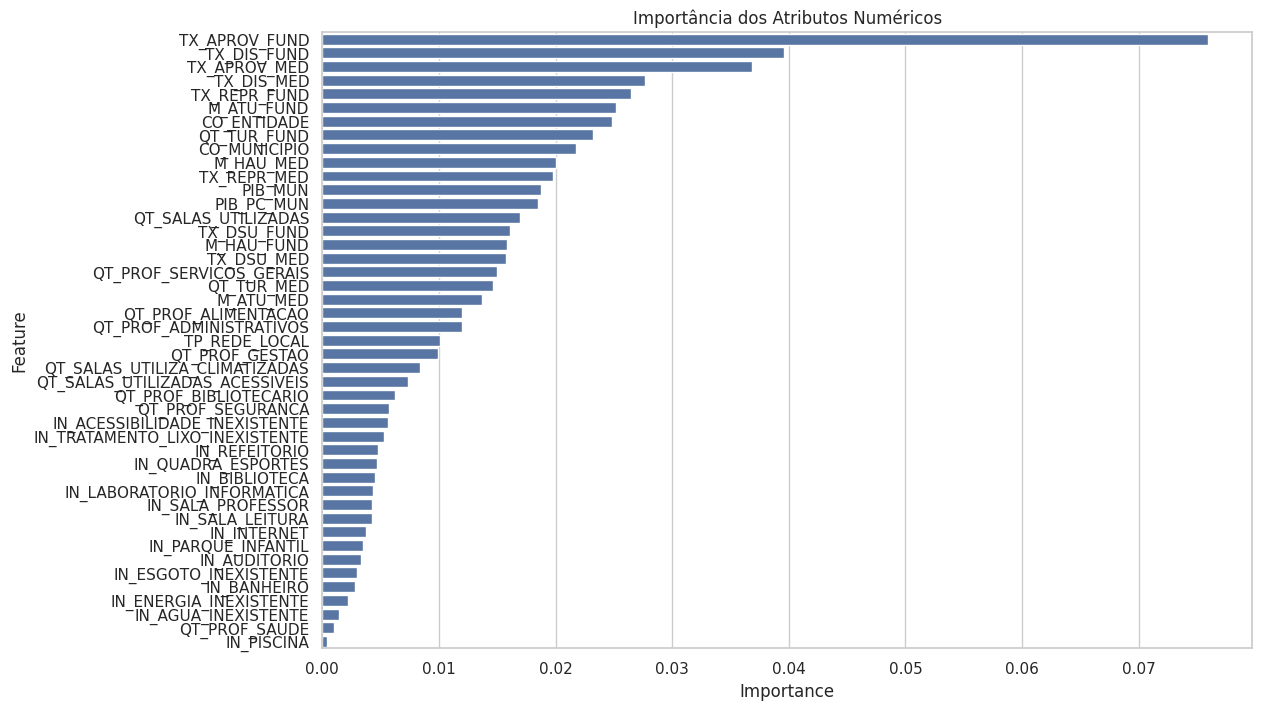
\includegraphics[scale = 0.4]{Graphics/Import-Ale.png}
    \caption{Importância dos atributos atribuídas pela Random Forest na amostragem aleatória.}
    \label{fig:enter-label}
\end{figure}

\par Assim, a partir das figuras, infere-se que as taxas de rendimento no ensino fundamental apresentaram uma relevância consideravelmente elevada na identificação de entidades escolares vulneráveis. Portanto, a fim de se combater os problemas de evasão escolar no território nacional, uma medida de suma importância é o investimento na educação basilar, ou seja, voltar as atenções para o ensino fundamental pois, a partir dele, um aluno pode adquirir condições de progredir educacionalmente.

\subsection{Comparação entre algoritmos}

\subsubsection{Random Forest}

\par O algoritmo da Random Forest, apesar de fornecer uma interpretação mais simples e intuitiva do resultado por meio da importância de cada atributo, resultou em um modelo com uma acurácia ligeiramente menor que o método de redes neurais. Desse modo, é razoável inferir que o modelo pode oferecer uma abordagem mais interpretável do modelo, porém, pode ser limitado pelo algoritmo e não oferecer um poder de generalização tão elevado.

\subsubsection{Redes neurais}

\par A partir das matrizes de confusão e das medidas do modelo, é possível concluir que o algoritmo apresentou um poder de generalização e de extração de conhecimento a partir dos dados maior, possibilitando obter recall e precisão maiores na modelagem.

\subsubsection{Comparação de métodos de amostragem}

\subsubsection{Amostra balanceada}

\par Com substrato lógico nos resultados dos modelos treinados a partir das amostras de dados balanceadas, é possível concluir que a etapa de treinamento a partir dessa amostra, justamente pela ausência de enviesamento por meio de uma classe majoritária no conjunto, proporcionou modelos mais sensíveis para identificar escolas com taxa de evasão alta e moderadas, aumentando o recall dessas categorias de escola, o que é o foco principal da problemática. Portanto, vê-se que, para que seja viável uma distinção mais bem definida de categorias de taxa de evasão escolar, priorizando as unidades educacionais realmente carentes, o treinamento em amostra balanceada se mostrou mais eficiente.

\subsubsection{Amostra aleatória}

\par A partir da saída dos modelos treinados em amostras aleatória, é razoável perceber que o enviesamento ocasionado pela classe majoritária, por mais que o modelo apresente uma acurácia geral maior, que tais estruturas não são suficientemente refinados no quesito de identificar escolas que realmente apresentam carência de ensino. Desse modo, conclui-se que as amostras não são tão efetivas para uma extração de conhecimento e reconhecimento de unidades de ensino vulneráveis, não sendo recomendada para ser base de uma pesquisa pública.

\subsection{Pesquisas relacionadas}

\par A respeito de pesquisas relacionadas à evasão escolar abordada com mineração de dados, no contexto brasileiro, podem ser encontradas tendo foco de análise a evasão escolar no ensino básico, a qual é estudada por \cite{sales2019evasao}, em que é utilizado o algoritmo WRF ou \textit{Weighted Random Forest} para prever a evasão escolar na cidade de Juiz de Fora em Minas Gerais. Os resultados dessa pesquisa foram obtidos após o algoritmo ser aplicado algumas vezes obtendo uma precisão média de 0.70 e um \textit{recall} médio de 0.97 nos seus atributo mais relevante.

\par Essa vertente de pesquisa também é desenvolvida em outras instâncias da educação brasileira como é o artigo apresentado por \cite{barbosa2023previsao} em que são utilizados dados de um dos campi do Instituto Federal de Pernambuco para fazer uma análise preditiva com base em cerca de 13 atributos dos alunos. Nessa pesquisa os melhores resultados obtidos foram utilizando do algoritmo \textit{Random Forest} obtendo 0.83 tanto na precisão quanto no \textit{recall} com uso de atributos sociodemográficos e acadêmicos.

\section{Discussões e decisões}

\subsection{Definição de intervalos de categorização do atributo alvo}

\par Também foram adotados como índices de evasão escolar os seguintes intervalos de valores: menor que 5\% como baixo, entre 5\% e 10\% como moderado e maior que 10\% como alto. Após pesquisar sobre o assunto, analisamos que esses valores como parâmetros de classificação são aceitáveis e condizem com a realidade.

\subsection{Imputação de dados}

\par A respeito do tratamento de dados faltantes, foi definido que a imputação por intermédio do algoritmo do KNN, com K igual a 5, seria uma estratégia válida devido à similaridade intraestadual dos municípios, preservando, assim, a fidelidade à realidade das unidades de ensino de uma mesma unidade federativa nacional.

\subsection{Proporção utilizada no método de amostragem}

\par Foi decidido que a utilização dos dados balanceados em detrimento dos desbalanceados seria mais benéfica dado que: para os dados balanceados, embora exista algumas predições incorretas quanto às evasões altas e moderadas, quando na realidade são baixas, o modelo prediz corretamente a grande maioria das evasões baixas. O problema surge nos dados desbalanceados, nos quais existem muitas predições baixas para evasões que são moderadas ou altas. Isso é grave, pois é muito importante que as evasões altas, principalmente, sejam preditas corretamente. Além disso, embora os modelos treinados na amostra aleatória apresentem maior acurácia geral, o recall da categoria de evasão alta foi mais elevado em modelos treinados na amostragem balanceada, o que prioriza as entidades alvo do estudo, as instituições de ensino vulneráveis e os fatores causadores de fragilidade.

\subsection{Algoritmo mais eficiente}

\par No estudo, foram analisados dois algoritmos para modelagem e, por fim, foi possível concluir que, apesar de uma interpretação e extração de parâmetros mais complexa, a rede neurais se mostrou mais eficiente em relação ao algoritmo da Random Forest graças ao seu poder de generalização mais refinado e uma maior sensibilidade a escolas mais fragilizadas.